\documentclass[final]{beamer}
\mode<presentation>{\usetheme{Berlin}}
%\documentclass[10pt, ]{beamer}
%\documentclass[10pt, handout]{beamer}
%\usepackage[orientation=portrait, size=a0, scale=1.25]{beamerposter}
\usepackage[orientation=portrait, size=a0, scale=1.0]{beamerposter}
%\usepackage{markdown} 
\usepackage[utf8]{inputenc}
\usepackage{multicol}
\usepackage{hyperref}
\usepackage{graphicx}
%\usepackage{color}
\usepackage{framed}
\usepackage{subcaption}
\usepackage{float}
\graphicspath{ {images/} }
\usepackage{blindtext}
\usepackage{mathtools}
\usepackage{amssymb}
\usepackage{amsfonts}
\usepackage{amsthm}
\usepackage[backend=biber]{biblatex}
\addbibresource{mybib.bib}
%\usepackage[dvipsnames]{xcolor}
\usepackage[section]{placeins} %\Floatbarrier
\usepackage{float}

%\usepackage[a4paper, width=150mm, top=25mm, bottom=25mm]{geometry}
\usepackage{fancyhdr}
%\setlength{\headheight}{12pt}
%\pagestyle{fancy}
%\pagestyle{empty}
\usepackage{lipsum}

%\usetheme{Madrid}
%\usetheme{Frankfurt}
%\mode<presentation>{\usetheme{Madrid}}
%\mode<presentation>{\usetheme{Berlin}}

%\title{GMMVAE model for scRNAseq}
\title{$\mathrlap{\ast}{C}$GMV\AE}
\subtitle{Classification, synthetic data generation and treatment effect
prediction}
\author{Yiftach Kolb and Martin Vingron}
\institute[FU and MPG]{
\centering
\vfill
{
\includegraphics[width=0.3\linewidth]{images/MPIMG_RGB_gruen.jpg}} %\\
%\hfill
%\vfill
\hspace{0.3cm}
{
\includegraphics[width=0.25\linewidth]{images/fu-logo_bildschirm_RGB1.jpg}}
}
%\institute1[MPG]{
%{
\includegraphics[width=0.2\linewidth]{images/MPIMG_Kompakt_RGB_gruen.jpg}} %\\
%}
%\institute2[FU Berlin]{
%{
\includegraphics[width=0.2\linewidth]{images/fu-logo_bildschirm_RGB1.jpg}}
%}
\date{\today}



\begin{document}

\begin{frame}[t]
\begin{block}
\maketitle
\end{block}
\begin{columns}


\begin{column}{0.50\textwidth}
\begin{block}{Abstract}
\begin{multicols}{3}
$\mathrlap{c}{\ast}$\\
$\mathllap{c}{\ast}$\\
$\mathclap{c}{\ast}$\\
$\mathrlap{\ast}{c}$\\
$\mathllap{\ast}{c}$\\
$\mathclap{\ast}{c}$\\
$\mathclap{\text{sC}}{\ast}$GMV\AE
The Gaussian Mixture VAE Model has been demonstrated to be a rather powerful 
model for unsupervised and (semi)supervised learning tasks on image
sets~\cite{dilokthanakul2016deep}.
We use a slightly modified and theoretically improved GMMVAE model and tested it on scRNAseq data.
We also tested a conditional version of our GMMVAE for the purpose of predicting
treatment effect on control cells of specific cell type.

Our results suggests that the GMMVAE in (semi)supervised learning is able to 
learn to both accurately classify and to generate the data.
synthetic data generation is one possible application.

As for prediction of treatment effect--- our cGMMVAE have similar results to one
method we compared~\cite{lotfollahi2018generative}.
\end{multicols}
\vspace{10cm}
\end{block}
\end{column}

\begin{column}{0.50\textwidth}
\begin{block}{GMMVAE models}
\begin{figure}[h]
\begin{subfigure}[b]{0.35\linewidth}
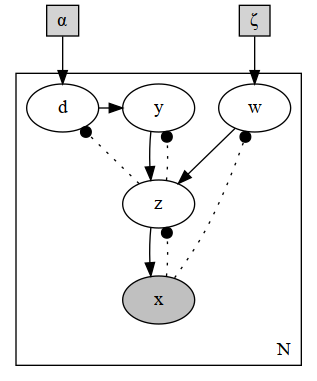
\includegraphics[width=0.92\linewidth]{plots/dirichlet_gmm.gv.png}
\caption{GMMVAE}
%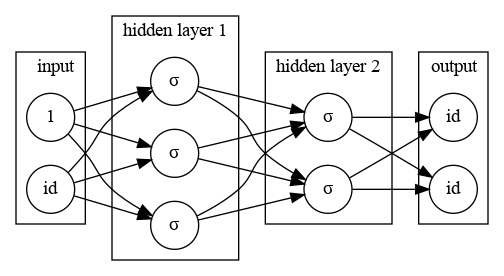
\includegraphics[width=0.8\textwidth]{./plots/neuronlayers.gv.png}

\end{subfigure}
\begin{subfigure}[b]{0.39\linewidth}
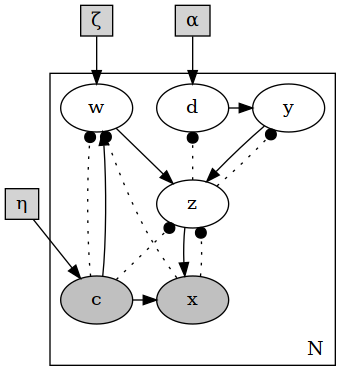
\includegraphics[width=0.97\linewidth]{./plots/dirichlet_gmm_cvae.gv.png}
%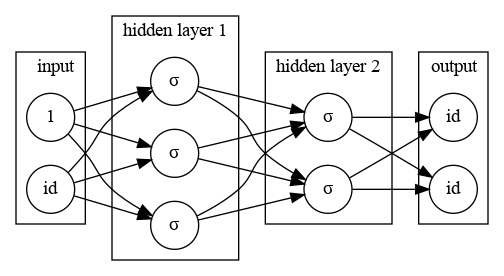
\includegraphics[width=0.8\textwidth]{./plots/neuronlayers.gv.png}
\caption{cGMMVAE}
\end{subfigure}
\end{figure}
\end{block}
\end{column}

\end{columns}


\begin{block}{Reference}
\printbibliography
\end{block}

\begin{block}{Abstract}
\begin{multicols}{3}[onlytextwidth]
%\begin{abstract}
The Gaussian Mixture VAE Model has been demonstrated to be a rather powerful 
model for unsupervised and (semi)supervised learning tasks on image
sets~\cite{dilokthanakul2016deep}.
We use a slightly modified and theoretically improved GMMVAE model and tested it on scRNAseq data.
We also tested a conditional version of our GMMVAE for the purpose of predicting
treatment effect on control cells of specific cell type.

%\lipsum
%\end{abstract}

\end{multicols}
\end{block}
\end{frame}

\begin{frame}[t]
%\begin{block}
%%title page
\begin{center}

\includegraphics[width=0.5\textwidth]{images/MPIMG_RGB_gruen.png}\\
%\vspace{1cm}
%%\vfill

\begin{block}

~ 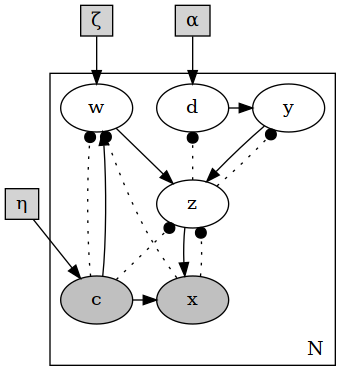
\includegraphics[width=0.22\linewidth]{plots/dirichlet_gmm_cvae.gv.png}

\Large
\textbf{GMMVAE model for scRNAseq
}
\vspace{0.5cm}
%%\normalsize


\large
Classification, synthetic data generation and treatment effect
prediction 
%
\includegraphics[width=0.4\textwidth]{images/MPIMG_RGB_gruen.png}

%%\vfill
\vspace{1.0cm}

Yiftach Kolb
%
\includegraphics[width=0.4\textwidth]{images/fu-logo_bildschirm_RGB1.jpg}
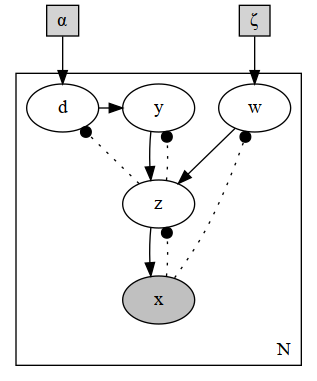
\includegraphics[width=0.22\linewidth]{plots/dirichlet_gmm.gv.png}
~
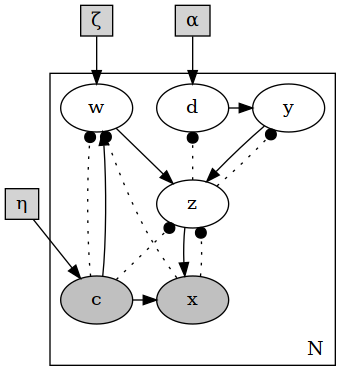
\includegraphics[width=0.22\linewidth]{plots/dirichlet_gmm_cvae.gv.png}

Berlin, \today

%%\vfill
\end{block}
%\vspace{1.0cm}


\includegraphics[width=0.5\textwidth]{images/MPIMG_RGB_gruen.png}
~

\includegraphics[width=0.4\textwidth]{images/fu-logo_bildschirm_RGB1.jpg}
%\normalsize
\end{center}
%\end{block}

\begin{block}{Abstract}
\begin{abstract}
the abstract.
\end{abstract}
\end{block}
\end{frame}

\begin{frame}[t]
\begin{block}
\maketitle
\end{block}
\begin{block}{Abstract}
\begin{abstract}
the abstract.
\end{abstract}
\end{block}
\begin{block}
%\begin{center}
%
\includegraphics[width=0.2\textwidth]{images/fu-logo_bildschirm_RGB1.jpg}

%\end{center}
\end{block}

\includegraphics[width=0.2\textwidth]{images/fu-logo_bildschirm_RGB1.jpg}
\begin{block}

\end{block}
\end{frame}

\begin{frame}[t]
\frametitle{frame title: Spam}

\begin{block}
\maketitle
%\titlepage
\end{block}

\begin{block}{bar}
foo

\end{block}


\begin{block}{barbi}
\fcolorbox{gray}{brown}{\textcolor{cyan}{test color}}
\end{block}

\begin{multicols}{3}[onlytextwidth]

\hrulefill\\
\pagecolor{purple}{
\fcolorbox{teal}{olive}{\textcolor{magenta}{test color \hrulefill}}\\
\hrulefill\\
}

\begin{block}{barbiiii}
another block
\end{block}

%\section{Intro}
%\title{Introduction}
Spam~\footfullcite{russkikh2020style} is good.
%\end{frame}
%\rule
\lipsum[0]

%\hrule

%\begin{frame}
And now to something~\cite{guo2017improved} completely different \dots


foo ...
foo ...
foo ...

foo ...
foo ...
foo ...

%\section{foo}
\lipsum[1]
foo ...
foo ...
foo ...

\lipsum[2]

%\section{bar}

\lipsum[3]

\lipsum[4]

\lipsum[5-8]

%\section{Reference}
%\printbibliography

foo ...
foo ...
foo ...

\end{multicols}

\begin{block}{multicols block}
\begin{multicols}{3}[onlytextwidth]
\lipsum[1-4]
\end{multicols}
\end{block}
\end{frame}


\begin{frame}[t]{manual column setting}
\begin{block}
\maketitle
%\titlepage
\end{block}
\begin{columns}

\begin{column}{0.50\textwidth}
\begin{block}{block headline}
\lipsum
\end{block}
\end{column}

\begin{column}{0.50\textwidth}
\begin{block}{block headline0}
\lipsum[1]
\end{block}

\begin{minipage}[c]{.65\textwidth}
\hrule
this is a 
minipage

lalalal
\end{minipage}

\begin{block}{block headline1}
\lipsum[1]
\end{block}

\begin{block}{block headline2}
\lipsum[2]
\end{block}


\end{column}
\end{columns}

\end{frame}




\end{document}
